\section{Auswertung}
\label{sec:Auswertung}
Für die Auswertung wurden NumPy \cite{numpy}, Matplotlib \cite{matplotlib}, SciPy \cite{scipy} und Uncertainties \cite{uncertainties} verwendet.

\subsection{Kraftflussdichte}
Die mithilfe einer Hall-Sonde ermittelte maximale Kraftflussdichte des Magnetfelds bei maximaler Stromstärke beträgt
\begin{equation*}
    B = \SI{392}{\milli\tesla}.
\end{equation*}
Diese Kraftflussdichte wird in der Mitte des Luftspalts des Elektromagneten erreicht.

\subsection{Effektive Masse mittels Faraday-Rotation}
Die Werte für die Dicke und die Donatorenkonzentration für die drei Proben sind in Tab. \ref{tab:proben} zu finden.
\begin{table} \caption{Die Werte für die Dicken und die Donatorenkonzentrationen für die reine GaAs-Probe und die beiden n-dotierten GaAs-Proben.}
    \label{tab:proben}
    \centering
    \sisetup{round-mode = places, round-precision=2, round-integer-to-decimal=true}
    \begin{tabular}{S[] S[] S[] S[]}
        \toprule
        {} & {Reine Probe} & {Probe 1} & {Probe 2} \\
        \midrule
        \text{Dicke} $d / \si{\milli\meter}$ & 5.11 & 1.296 & 1.36 \\
        \text{Donatorendichte} $N / \si[per-mode=reciprocal]{\per\cubic\centi\meter}$ &  & 0.28e19 & 0.12e19 \\
        \bottomrule
    \end{tabular}
\end{table}

Die eingestellten Winkel bei den verschiedenen Wellenlängen stehen in Tab. \ref{tab:winkel}.

\begin{table} \caption{Winkel.}
    \label{tab:winkel}
    \centering
    \sisetup{round-mode = places, round-precision=2, round-integer-to-decimal=true}
    \begin{tabular}{S[] c c c c c c}
        \multicolumn{1}{c}{$\lambda / \si{\micro\meter}$} & \multicolumn{2}{c}{Reine Probe} & \multicolumn{2}{c}{Probe 1} & \multicolumn{2}{c}{Probe 2} \\
        \cmidrule(l){2-3} \cmidrule(l){4-5} \cmidrule(l){6-7}
       {} & {$\theta_1$} & {$\theta_2$} & {$\theta_1$} & {$\theta_2$} & {$\theta_1$} & {$\theta_2$} \\
        \midrule
1.06  &  90°  40' &  66° 18' & 83° 40' & 72° 09'  & 83°  0' & 73° 23'\\
1.29  &  85°  13' &  69° 20' & 80° 25' & 71° 29'  & 80° 45' & 73° 15'\\
1.45  &  84°  50' &  72° 0'  & 81°  0' & 72° 30'  & 81°  0' & 74° 11'\\
1.72  &  80°  15' &  71° 19' & 79°  0' & 69° 23'  & 78° 12' & 72° 12'\\
1.96  &  72°  29' &  66° 38' & 78° 10' & 62° 13'  & 71° 47' & 65° 18'\\
2.156 &  71°   0' &  65° 10' & 72° 14' & 60° 25'  & 70° 42' & 64°  0'\\
2.34  &  46°  24' &  43° 5'  & 51° 12' & 37° 19'  & 47° 30' & 40° 25'\\
2.51  &  23°  30' &  29° 0'  & 29°  8' & 22° 18'  & 34° 00' & 21° 10'\\
2.65  &  63°  10' &  56° 34' & 70°  1' & 56°  0'  & 65° 27' & 57° 18'\\
        \bottomrule
    \end{tabular}
\end{table}

Die aus den Winkeln aus Tab. \ref{tab:winkel} mit \ref{eq:rotation} berechneten Rotationswinkel befinden sich in Tab. \ref{tab:skaliert}.

\begin{table} \caption{Winkel.}
    \label{tab:skaliert}
    \centering
    \sisetup{round-mode = places, round-precision=2, round-integer-to-decimal=true}
    \begin{tabular}{cccc}
        \toprule
        {$\lambda / \si{\micro\meter}$} & {$\theta_\text{rein}/ \si{\degree}$} & {$\theta_1/ \si{\degree}$} & {$\theta_2/ \si{\degree}$} \\
        \midrule
     1.06 &  41.61 &  77.54   &   61.71 \\
     1.29 &  27.12 &  60.15   &   48.12 \\
     1.45 &  21.91 &  57.23   &   43.74 \\
     1.72 &  15.25 &  64.75   &   38.50 \\
     1.96 &  9.99  &  107.39  &   41.60 \\
     2.156&  9.96  &  79.56   &   42.99 \\
     2.34 &  5.66  &  93.48   &   45.45 \\
     2.51 &  -9.39 &  46.01   &   82.35 \\
     2.65 &  11.27 &  94.38   &   52.30 \\
        
        \bottomrule
    \end{tabular}
\end{table}

Die quadrierte Wellenlänge ist in Abb. \ref{fig:alle} gegen die in Tab. \ref{tab:skaliert} stehenden Werte aufgetragen.
\begin{figure}
    \centering
    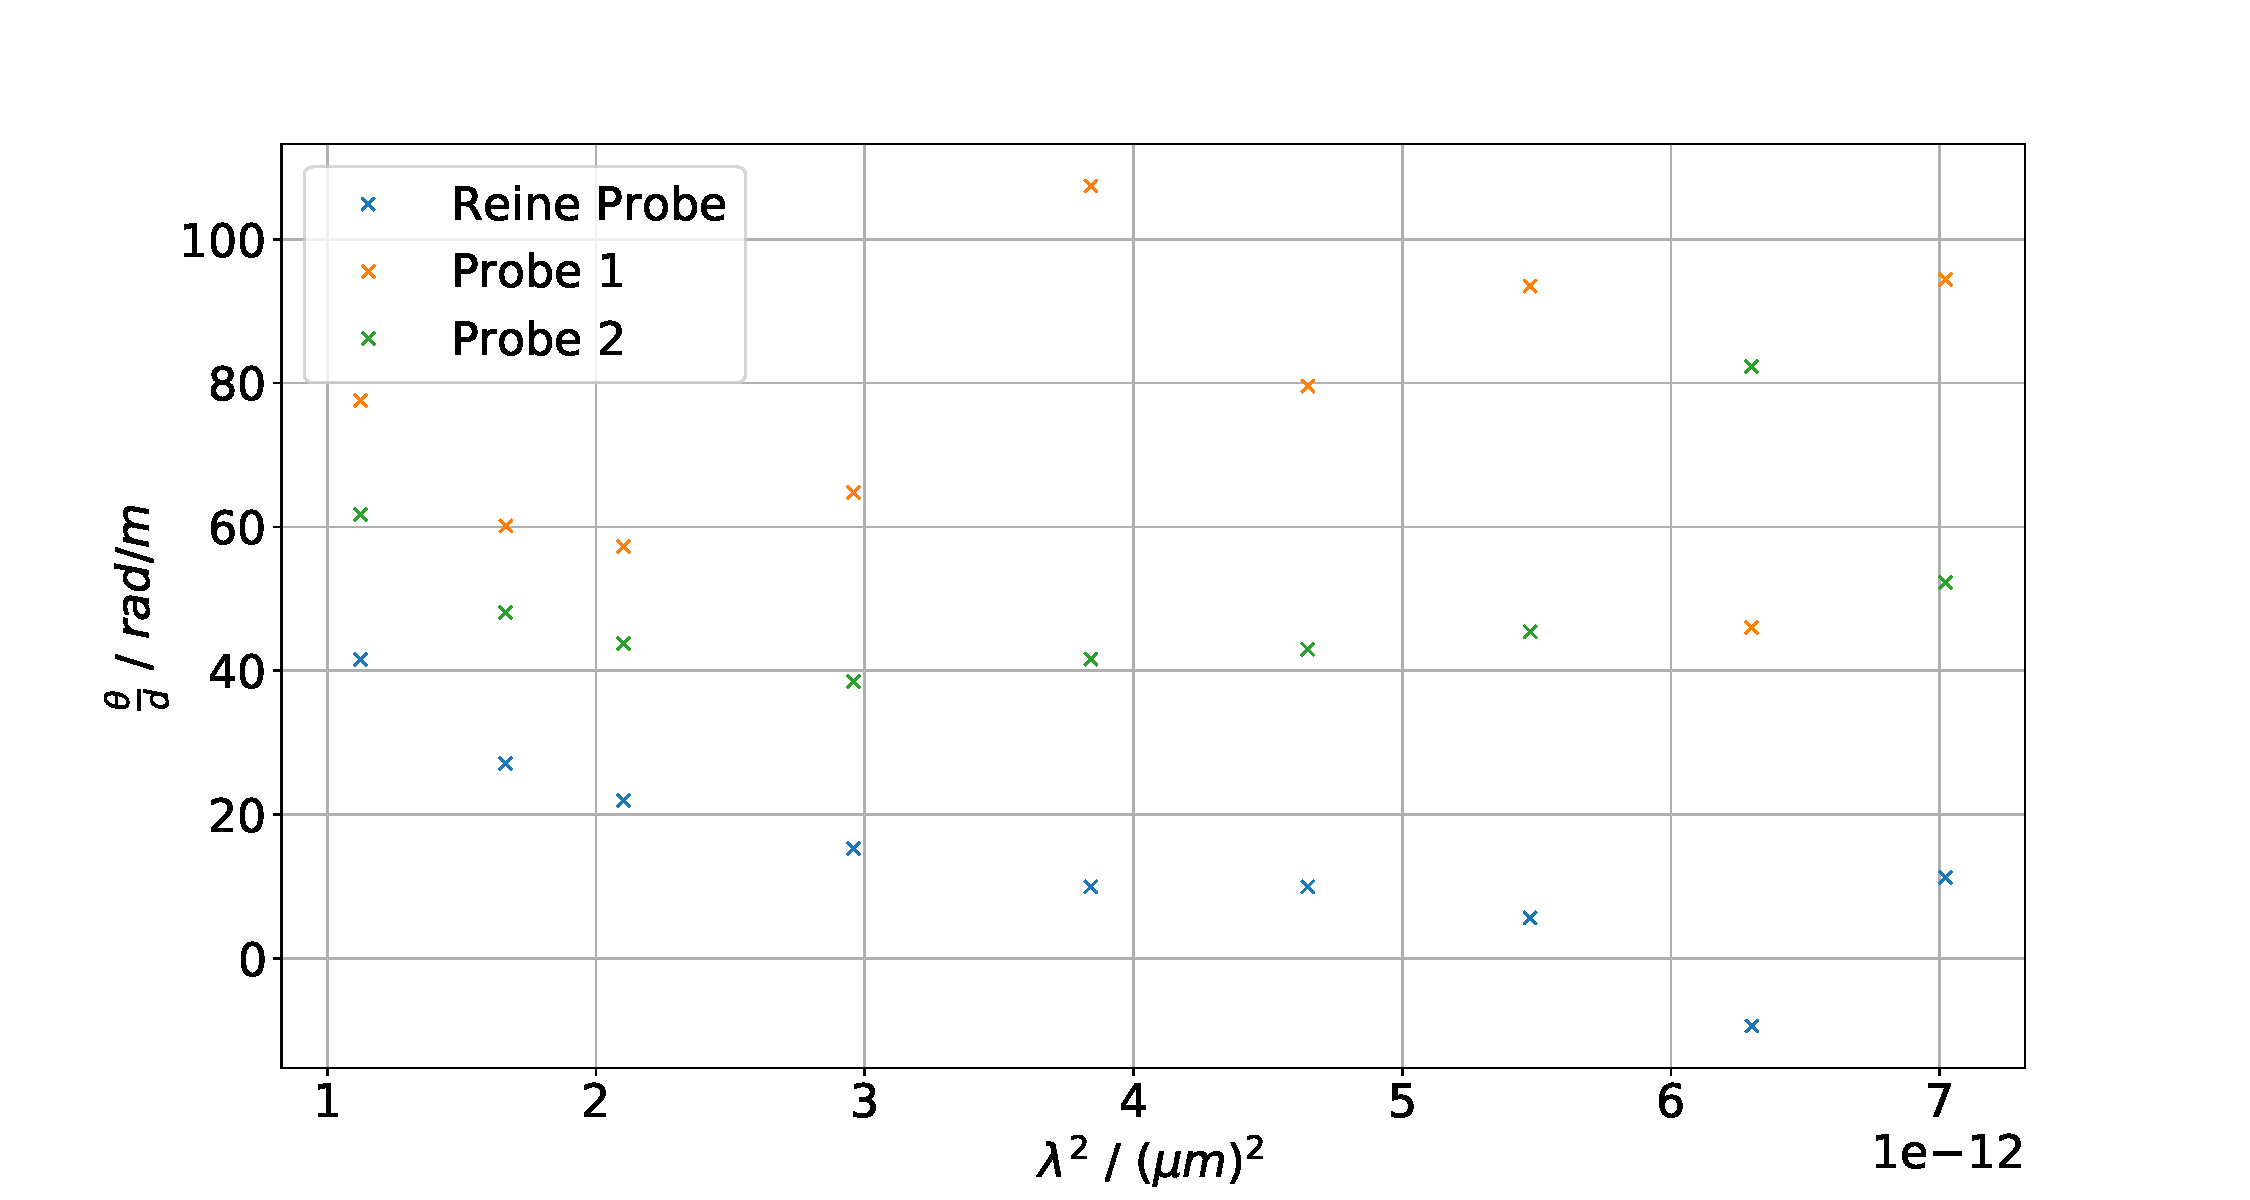
\includegraphics[width=15cm]{plots/AlleProben.pdf}
    \caption{Die Rotationswinkel der reinen und der beiden n-dotierten Proben sind gegen die quadratische Wellenlänge aufgetragen.}
    \label{fig:alle}
\end{figure}

Zur Bestimmung der effektiven Masse wird jeweils der Betrag der Differenz des Rotationswinkels der reinen Probe und des Rotationswinkels der dotierten Probe gebildet. Diese Werte sind in Tab. \ref{tab:frei} eingetragen.

\begin{table} \caption{Winkel.}
    \label{tab:frei}
    \centering
    \sisetup{round-mode = places, round-precision=2, round-integer-to-decimal=true}
    \begin{tabular}{S[] S[] S[]}
        \toprule
        {$\lambda / \si{\micro\meter}$} & {$\theta_\text{rein}/ \si{\degree}$} & {}
        \midrule
1.06    & 35.93  & 20.09 \\
1.29    & 33.02  & 20.99 \\
1.45    & 35.31  & 21.82 \\
1.72    & 49.49  & 23.24 \\
1.96    & 97.40  & 31.61 \\
2.156   & 69.60  & 33.02 \\
2.34    & 87.81  & 39.78 \\
2.51    & 55.40  & 91.73 \\
2.65    & 83.11  & 41.02 \\
        \bottomrule
    \end{tabular}}
\end{table}

Der Drehwinkel wird für beide Proben gegen $\lambda^2$ aufgetragen. Der Proportionalitätsfaktor zwischen den Größen wird bestimmt. Daraus wird die effektive Masse mit Gleichung \ref{eq:theta} berechnet. In Abb. \ref{fig:probe1} sind die Werte für Probe 1 zu sehen, in Abb. \ref{fig:probe2} die für Probe 2.
\begin{figure}
    \centering
    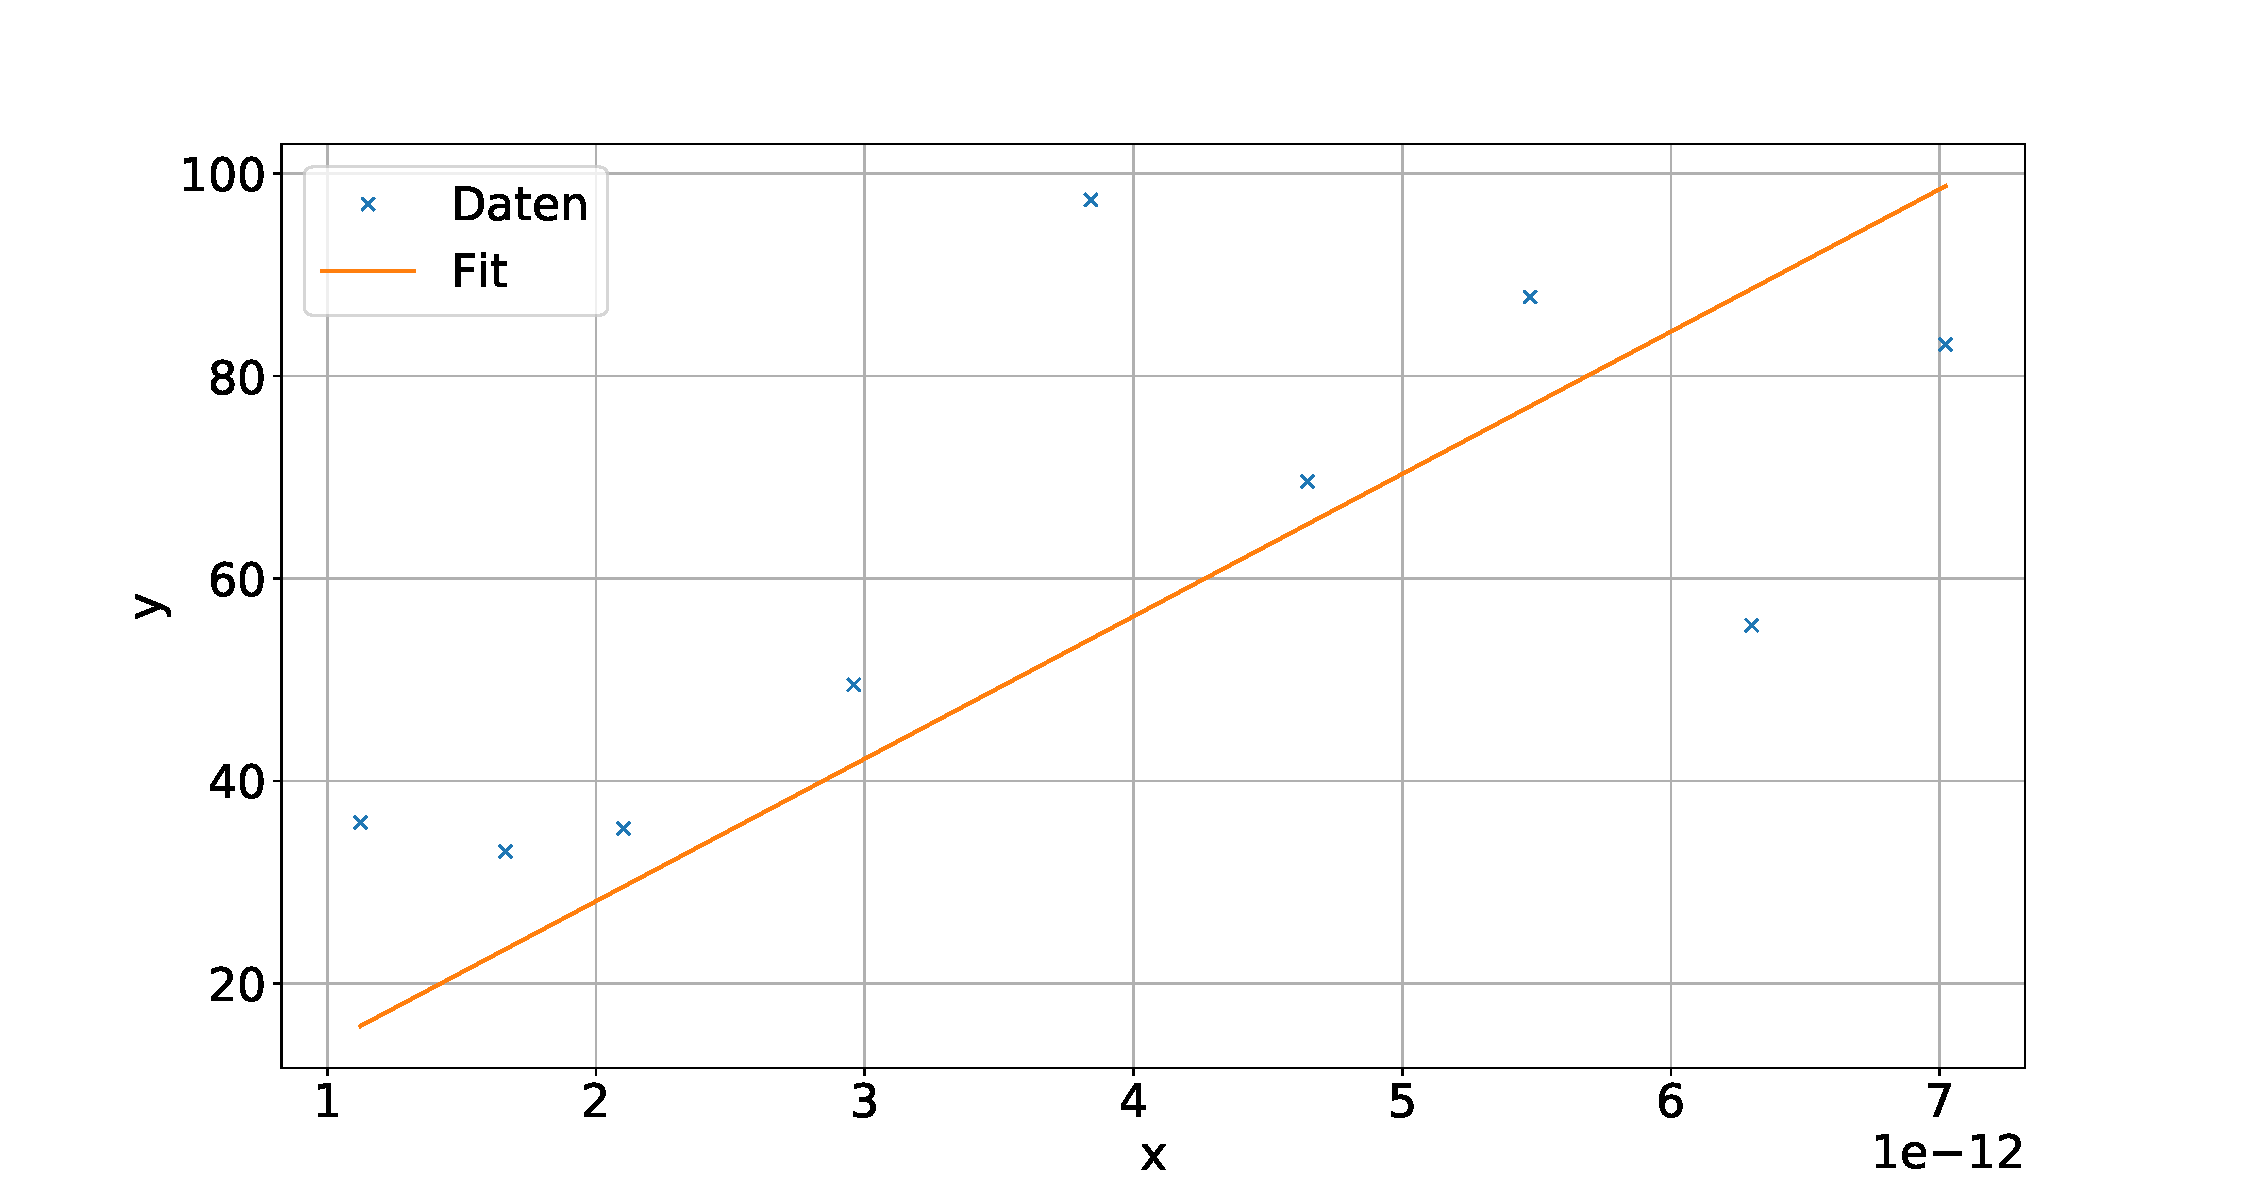
\includegraphics[width=15cm]{plots/Probe1.pdf}
    \caption{Die Differenz der Rotationswinkel von der reinen und der ersten n-dotierten Probe ist gegen die quadratische Wellenlänge aufgetragen. Zu sehen sind die Daten und eine Ausgleichsgerade.}
    \label{fig:probe1}
\end{figure}

\begin{figure}
    \centering
    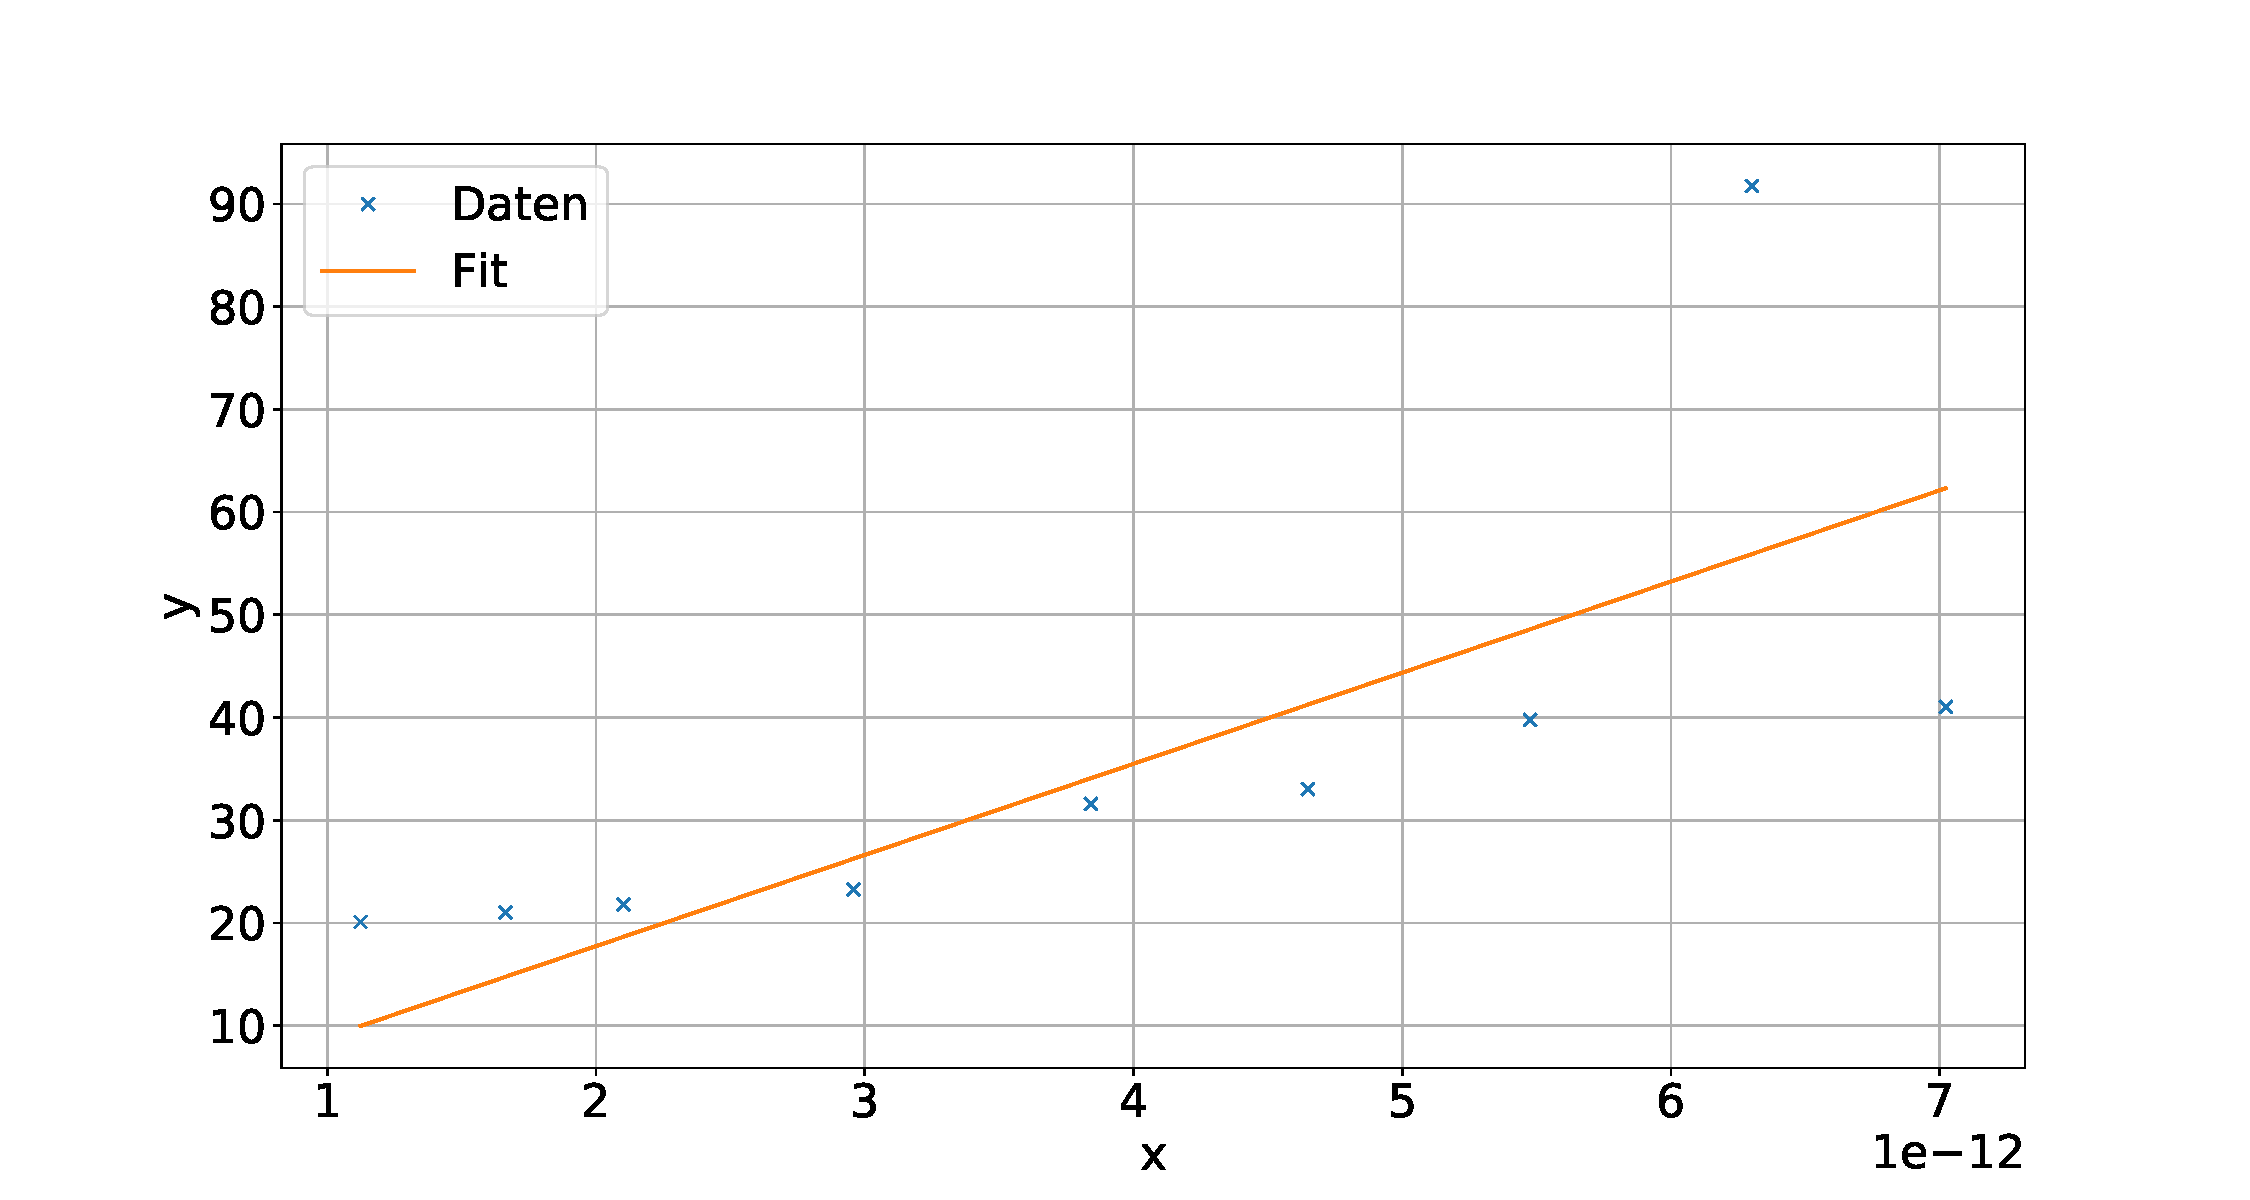
\includegraphics[width=15cm]{plots/Probe2.pdf}
    \caption{Die Differenz der Rotationswinkel von der reinen und der zweiten n-dotierten Probe ist gegen die quadratische Wellenlänge aufgetragen. Zu sehen sind die Daten und eine Ausgleichsgerade.}
    \label{fig:probe2}
\end{figure}

Im Folgenden steht die Zahl im Index für die Probe. Die Steigungen der Ausgleichsgeraden werden zu
\begin{align*}
    s_1 &= \SI{0}{\radian\per\cubic\meter} \\
    s_2 &= \SI{0}{\radian\per\cubic\meter}
\end{align*}
bestimmt. Daraus folgt für die effektiven Massen mit \ref{eq:theta}
\begin{align*}
    m_\text{eff,1} &= \num{0} \, m_\text{e} \\
    m_\text{eff,2} &= \num{0} \, m_\text{e},
\end{align*}
wobei $m_\text{e}$ die Elektronenmasse ist.